% !TeX spellcheck = en_US
% !TeX encoding = UTF-8
% !TeX root = ../document.tex

\chapter{Introduction}

This thesis deals with the \acf{MUSiC}, which is a particle physics analysis aiming to find new physics within data observed by the \acf{CMS} experiment.

In the first chapter, the \acl{SM} of particle physics and the \acs{CMS} experiment are introduced. 
The introduction is extended in the second chapter, which provides a description of the \acs{MUSiC} analysis in its current state. Different strategies and algorithms within the analysis framework are motivated and explained. Afterwards, the third chapter serves as a reference of simulations used within this thesis. The remaining chapters contain new contributions to the analysis: In the fourth chapter, the existing local test statistic \TS is evaluated and a possible alternative are discussed. Additionally, a global measure for the discovery potential is introduced. It is used in the final chapter, where simulations of new physics processes are used to assess the discovery potential of the aforementioned methods. 

\section{Units and Abbreviations}
Throughout this work, we will use the natural unit system. This means that the speed of light and the Planck constant are fixed to $1$:
\begin{equation*}
    \hbar = c = 1
\end{equation*}
It follows that the only unit needed to express most other physical quantities is the unit of energy. Our choice here is electron volts. Too keep numbers in a reasonable range, we mostly use gigaelectronvolts: $\SI{1}{\giga\eV} = \SI{1e9}{\eV} = \SI{1.60218e-10}{\joule}$.
Two exceptions to this are the cross section and luminosity, which are expressed in femtobarn and inverse femtobarn respectively: $\SI{1}{\femto\barn} = \SI{e-43}{\meter\squared}$.

\section{The Standard Model}
Finding substructure of matter has interested mankind for thousands of years. Ancient Greek philosophers already contemplated about the basic building blocks of matter\cite{Melsen:atomosatomhistory}. They coined the term \emph{atom} for what they thought to be indivisible. Since then, our understanding of the smallest parts and what holds them together has vastly improved. This field of science is nowadays called \emph{Elementary Particle Physics}. 

As of 2017, the most broadly accepted model in particle physics is the so-called \emph{\acl{SM} of Particle Physics}. The \acl{SM} describes matter and its interactions through \emph{particles} and \emph{forces}. It is based on the mathematical foundation of quantum field theory, exhibiting several concepts such as gauge invariance, spontaneous symmetry breaking, perturbative and non-perturbative behavior.
 
Although it has provided accurate predictions, making it a successful theory, recent observations have yielded some inconsistencies, which motivate the scientific field to advance. The following sections will be a short introduction to the \acl{SM}, its historical development, fundamental ideas and open questions. Motivated by these questions, possible extensions to the \acl{SM} will be introduced afterwards.

\subsection{Particles and Interactions}
Elementary particles are described as point-like indivisible structureless objects, much like the atoms were to the ancient Greeks. These objects are characterized by physical observables such as mass, charge and spin.

Elementary particles can be subdivided into several groups, as shown in \fref{fig:particle_groups}. 
At the first level, one distinguishes between two groups: \emph{fermions} and \emph{bosons}.

\begin{figure}
    \centering
%    \includegraphics[width=0.5\textwidth]{Elementary_particle_interactions}
    \tikzset{font=\small,
        edge from parent fork down,
        level distance=3em,
        sibling distance=0.3em,
        every node/.style=
        {
            align=center,
        },
        every leaf node/.style={
            circle,
            draw,           
            very thick,
            inner sep=0,
            minimum size=1.4em,
            text height=0.5em,
            text depth=0,
        }
    }
    \begin{tikzpicture}
    \Tree
    [.{Elementary Particles}
        [.Fermions
            [.Leptons
                [.{charged}
                    {\Pe}
                    {\Pmu}
                    {\Ptau}
                ]
                [.{neutrinos}
                    {\Pnue}
                    {\Pnum}
                    {\Pnut}
                ]
            ]
            [.Quarks
                [.{up-type}
                    {\Pup}
                    {\Pcharm}
                    {\Pbottom}
                ]
                [.{down-type}
                    {\Pdown}
                    {\Pstrange}
                    {\Ptop}
                ]
            ]
        ]
        [.Bosons
            {\Pgamma}
            {\Pgluon}
            [.{charged}
                {\PW}
                {\PZ}
            ]
            {\PHiggs}
        ]
    ]
    \end{tikzpicture}
    \caption{Nested groups of elementary particles. The actual particle symbols are indicated by circles.}
    \label{fig:particle_groups}
\end{figure}

Fermions are elementary particles with a spin of $\nicefrac{1}{2}$. They follow Fermi-Dirac statistics and have to obey Pauli's exclusion principle which states that no more than one particle can occupy a certain state characterized by its quantum numbers.
The group of fermions can be further divided into \emph{quarks} and \emph{leptons}.
There are six quarks: up (\Pup), down (\Pdown), charm (\Pcharm), strange (\Pstrange), bottom (\Pbottom) and top (\Ptop). Quarks carry color charge and are the only fermions to take part in the strong interaction.
The remaining fermions are called leptons. There are three charged leptons: The \emph{electron} (\Pe), the \emph{muon} (\Pmu) and the \emph{tau} (\Ptau). Each of the charged leptons has a massless, electrically neutral \emph{neutrino} (\Pnue, \Pnum, \Pnut), associated with it.

The second group of particles are called bosons. They mediate interactions (also called \emph{forces}) and possess an integer spin. Bosons follow Bose-Einstein statistics and may thus occupy the same quantum state.
Each kind of boson is responsible for one kind of elementary force: the electrodynamic force is mediated by the \emph{photon} (\Pgamma), the strong force by the \emph{gluon} (\Pg) and the weak force by the \emph{\PZ} and \emph{\PW} bosons.
In addition, there is the \emph{Higgs boson} (\PH), which uses the Higgs mechanism to give mass to all mentioned massive elementary particles.\footnote{Note that this does not apply to composite particles (like protons) which gain mask mostly through binding energy.}

\begin{table}
    \centering
    \begin{tabular}{l r s[table-unit-alignment = left]}
        \toprule
        Lepton & \multicolumn{2}{l}{Mass} \\
        \midrule
        \Pe & 511 & \keV \\
        \Pnue & < 2 & \eV \\
        \Pmu & 106 & \MeV \\
        \Pnum & < 2 & \eV \\
        \Ptau & 1.78 & \GeV \\
        \Pnut & < 2 & \eV \\
        \bottomrule
    \end{tabular}
    \begin{tabular}{l r s[table-unit-alignment = left]}
        \toprule
        Quark & \multicolumn{2}{l}{Mass} \\
        \midrule
        \Pup & 2 & \MeV \\
        \Pdown & 5 & \MeV \\
        \Pcharm & 1.3 & \GeV \\
        \Pstrange & 96 & \MeV \\
        \Pbottom & 4.18 & \GeV \\
        \Ptop & 173 & \GeV \\
        \bottomrule
    \end{tabular}
    \begin{tabular}{l r s[table-unit-alignment = left]}
        \toprule
        Boson & \multicolumn{2}{l}{Mass} \\
        \midrule
        \Pgamma & 0 &  \\
        \Pgluon & 0 &  \\
        \PW & 80.4 & \GeV \\
        \PZ & 91.2 & \GeV \\
        \PH & 125 & \GeV \\
        \bottomrule
    \end{tabular}
    \caption{Known elementary particles and their masses\cite{ParticleDataGroup:ReviewParticlePhysics}.}
    \label{tab:particles}
\end{table}

\subsection{Interactions}
\subsubsection{Quantum Electrodynamics}
The theory of electromagnetism at extremely small or extremely high energetic scales is called \acfi{QED}. It is a field theory that unifies classical quantum mechanics, special relativity and gauge invariance.

Because the probability amplitude of a quantum mechanical wave function is independent of the wave's phase, two wave functions that only differ in phase are equivalent. Thus, physics processes should behave exactly the same, regardless of the phase term. This concept is called \emph{invariance under phase transformations} and is a desirable property for quantum field theories.

In 1928, the British physicist Paul Dirac derived an relativistic extension of the classical Schrödinger equation\cite{Dirac:quantumtheoryelectron} by substituting observables with corresponding operators in the relativistic energy-momentum relation $E^2 = p^2 + m^2$. The resulting so-called \emph{Dirac equation} describes the behavior of free spin-\nicefrac{1}{2} particles and even predicts the existence of antiparticles.
However, the Dirac equation is not invariant under phase transformations and thus Richard Feynman et al. developed a gauge invariant extension of Dirac's theory\cite{Feynman:Spacetimeapproach}. This extension, quantum electrodynamics, was awarded the Nobel Prize in 1965\cite{NobelMedia:NobelPrize1965}.

The theory of \ac{QED} evolves around the photon coupling to the electric charge $e$: The photon interacts with charged particles with a strength of $\alpha \propto e^2$.
All possible basic vertices are displayed in \fref{fig:qed_vertices}: Two charged particles may annihilate into one photon, a photon may be emitted or absorbed, or an oppositely charged particle-antiparticle pair may be created from the photon energy. Note that in any case, the electric charge as well as the fermion type are preserved.

\begin{figure}
    \centering
    \begin{fmffile}{qed_basic_1}
        \begin{fmfgraph*}(3,3)
            \fmfleft{f2,f1}
            \fmf{fermion,label=\Pf}{f1,i}
            \fmf{fermion,label=\Paf}{i,f2}
            \fmf{photon,label=\Pphoton}{l,i}
            \fmfright{l}
        \end{fmfgraph*}
        \hspace{1cm}
        \begin{fmfgraph*}(3,3)
            \fmfleft{f1}
            \fmfright{f2}
            \fmf{fermion,label=\Pf}{f1,i}
            \fmf{fermion,label=\Pf}{i,f2}
            \fmf{photon,label=\Pphoton}{l,i}
            \fmfforce{(0,0)}{f1}
            \fmfforce{(w,0)}{f2}
            \fmftop{l}
        \end{fmfgraph*}
        \hspace{1cm}
        \begin{fmfgraph*}(3,3)
            \fmfleft{l}
            \fmf{fermion,label=\Paf}{f1,i}
            \fmf{fermion,label=\Pf}{i,f2}
            \fmf{photon,label=\Pphoton}{l,i}
            \fmfright{f2,f1}
        \end{fmfgraph*}
    \end{fmffile}
    \caption{Basic interaction vertices of \ac{QED}: Annihilation of a particle-antiparticle pair into one photon, emission or absorption of a photon, pair production from photon energy. The time direction is from left to right. Note that for kinetic reasons, these vertices cannot exist on their own, but are part of larger diagrams.}
    \label{fig:qed_vertices}
\end{figure}

One challenge that arises during the calculation of interaction probabilities for a particular \ac{QED} process is that one has to take into account all possible scenarios that lead to the same indistinguishable result. This includes diagrams containing fermion or photon loops, as shown in \fref{fig:qed_higher_order}. In order to calculate the scattering amplitude for this particular example, one has to integrate over all possible momenta $k$ within the loop. Unfortunately, this integral diverges quickly. A solution for this problem is \emph{renormalization}: By making the coupling strength $\alpha(q^2)$ dependent on the momentum transfer, infinities can be avoided. $\alpha(q^2)$, which now "runs" with the momentum transfer is consequently called \emph{running coupling constant}. Its value is $\alpha(0) \approx \frac{1}{137}$ in the low energy limit and increases towards higher energies\cite{Halzen:Quarksleptonsintroductory}. 

\begin{figure}
    \centering
    \begin{fmffile}{qed_higher_order}
        \begin{fmfgraph*}(7,4)
            \fmfleft{o1,i1}
            \fmfright{o2,i2}
            \fmf{fermion,tension=0.5,label=$p_1$}{i1,v1,o1}
            \fmf{fermion,tension=0.5,label=$p_2$}{i2,v2,o2}
            \fmf{photon,label=$q$}{v1,x1}
            \fmf{fermion,left,tension=0.5,label=$k$}{x1,x2}
            \fmf{fermion,left,tension=0.5,label=$q - k$}{x2,x1}
            \fmf{photon,label=$q$}{x2,v2}
        \end{fmfgraph*}
    \end{fmffile}
    \caption{Higher order Feynman diagram of electron-positron annihilation. Renormalization is required because of divergence of the integral over $k$.}
    \label{fig:qed_higher_order}
\end{figure}

\subsubsection{Quantum Chromodynamics}
After \ac{QED}, the theory of \acfi{QCD} was proposed in the early 1960s, as bubble chamber experiments had unexpectedly discovered large numbers of hadrons with different masses and physical properties. 
Instead of assuming that these particles were fundamental, theorists Murray Gell-Mann et al. proposed a theory where they were made up of constituents, so-called quarks\cite{Gell-Mann:EightfoldWayTheory,Gell-Mann:SchematicModelBaryons}. 
The theory of bound states of the three known quarks (\Pqu, \Pqd, \Pqs) and their excitations was able to reproduce many of the observations.
However, the observed $\Updelta^\text{++}$ baryon seemed to violate Pauli's exclusion principle: It consists of three \Pqu quarks with parallel spins. This dilemma was resolved in 1964, when Oscar W. Greenberg proposed a new quantum number, called \emph{color charge}\cite{Greenberg:SpinUnitarySpin}.
Alongside this quantum number, the existence of a gauge boson was predicted, the gluon, which was discovered at \acs{DESY} in 1979 in three-jet events\cite{Barber:DiscoveryThreeJet}.

The basic interaction vertices of \ac{QCD} are shown in \fref{fig:qcd_vertices}. The charge of the strong interaction is called color-charge, its possible values are usually called \emph{red}, \emph{green}, \emph{blue}, antired, antigreen and antiblue\footnote{Note that this concept is completely unrelated to visual perception of color.}.
Quarks carry one unit of color charge, while gluons carry two units. Color charge is conserved within each interaction vertex. 
An important principle of \ac{QCD} is that all naturally occurring particles are colorless: A composite particle carries either all colors (red + green + blue) or a color and its anti-color (e.g. red + antired). The former is found in baryons and the latter in mesons.

\begin{figure}
    \centering
    \begin{fmffile}{qcd_basic_1}
        \begin{fmfgraph*}(3,3)
            \fmfleft{f1}
            \fmfright{f2}
            \fmf{fermion,label=\Pq}{f1,i}
            \fmf{fermion,label=\Pq}{i,f2}
            \fmf{gluon,label=\Pg}{l,i}
            \fmfforce{(0,0)}{f1}
            \fmfforce{(w,0)}{f2}
            \fmftop{l}
        \end{fmfgraph*}
        \hspace{1cm}
        \begin{fmfgraph*}(3,3)
            \fmfleft{f1}
            \fmfright{f2}
            \fmf{gluon,label=\Pg,label.side=left}{f1,i}
            \fmf{gluon,label=\Pg,label.side=right}{i,f2}
            \fmf{gluon,label=\Pg}{l,i}
            \fmfforce{(0,0)}{f1}
            \fmfforce{(w,0)}{f2}
            \fmftop{l}
        \end{fmfgraph*}
        \hspace{1cm}
        \begin{fmfgraph*}(3,3)
            \fmfleft{f1,f2}
            \fmfright{f3,f4}
            \fmf{gluon,label=\Pg,label.side=left}{f1,i}
            \fmf{gluon,label=\Pg,label.side=right}{f2,i}
            \fmf{gluon,label=\Pg,label.side=left}{i,f3}          
            \fmf{gluon,label=\Pg,label.side=right}{i,f4}
            \fmfforce{(0,0)}{f1}
            \fmfforce{(0,h)}{f2}
            \fmfforce{(w,0)}{f3}
            \fmfforce{(w,h)}{f4}
        \end{fmfgraph*}
    \end{fmffile}
    \caption{Basic interaction vertices of the strong force: Absorption or emission of a gluon from a quark, self interactions between gluons. Note that each diagram can be read in different directions, similarly to \fref{fig:qed_vertices}.}
    \label{fig:qcd_vertices}
\end{figure}

Similarly as with \ac{QED}, \ac{QCD} also has to undergo renormalization. But unlike \ac{QED}, where only fermionic loops are possible, gluons can also interact with each other, resulting in gluon loops. Therefore, renormalization in \ac{QCD} is much more complicated. Its result is again a running coupling constant, however this time, the strong coupling constant $\alpha_s(q^2)$ decreases at higher energies. In fact, at infinite energies the quarks appear to be free, therefore this effect is called \emph{asymptotic freedom}.

The contrary effect at low energies is also visible: As the distance between quarks is increased, which is equivalent to decreasing the probing energy, the coupling strength rises. The expended energy in turn allows new quark-antiquark pairs to form from the vacuum. Each of the created quarks binds with one of the separated quarks such that all quarks again end up in a bound, color-neutral state. This effect tis called \emph{confinement}.

Confinement is also relevant in the experimental context: Quarks and gluons in the final state of a collision often posses excess kinetic energy and thus move away from each other. During that process, confinement causes new quarks and eventually hadrons to form. This effect is called \emph{hadronization}. Repeated hadronization leads to the formation of so-called \emph{jets}, cones of hadrons and subsequent decay products.


\subsubsection{Electroweak Interaction}
Although theoretical research on the \emph{weak interaction} started in 1933 when Enrico Fermi proposed a contact interaction theory explaining the $\upbeta$-decay\cite{Fermi:Tentativodiuna}, it was only further explored in the second half of the 20th century. 

In 1968, Sheldon Glashow\cite{Glashow:PartialSymmetriesWeak}, Abdus Salam\cite{Salam:WeakElectromagneticInteractions} and Steven Weinberg\cite{Weinberg:modelleptons} independently formulated a theory unifying \ac{QED} with the weak interaction, called \emph{electroweak theory}. They discovered that instead of classifying particles by their type and electrical charge, they could be regarded by quantum numbers called \emph{weak isospin} and \emph{weak hypercharge}. The theory introduces four gauge fields, $W_1$, $W_2$, $W_3$ and $B$ which couple to these charges. It then predicts the existence of four bosons: The charged massive \PWp and \PWm, which directly correspond to the fields $W_1$ and $W_2$ and the massive \PZ and massless photon which arise from mixing of the $W_3$ and $B$ fields. While the photon had been known for a long time, the predicted vector bosons were experimentally confirmed by Carlo Rubia's group at \acs{CERN}\cite{Arnison:ExperimentalObservationIsolated,Arnison:Experimentalobservationlepton} 15 years later.
The mixing angle used for the \PZ and photon is called \emph{Weinberg angle}, and in turn also relates the coupling strengths of the weak interaction and \ac{QED} with the electroweak couplings $g$ and $g'$\cite{Schleper:TeilchenphysikfuerFortgeschrittene}.

Besides \ac{QED}, the electroweak theory predicts the weak force, which is mediated by the heavy gauge bosons \PWpm and \PZ. The name "weak force" originates from its finite range and coupling strength which is much smaller than $\alpha$ or $\alpha_s$. Although the weak interaction would not be able to exist without electroweak unification, it is sometimes treated as a separate theory, called \acfi{QFD}.


\begin{figure}
    \centering
    \begin{fmffile}{qfd_basic_1}
        \begin{fmfgraph*}(3,3)
            \fmfleft{f1}
            \fmfright{f2}
            \fmf{fermion,label=\Pl}{f1,i}
            \fmf{fermion,label=\Pneutrino}{i,f2}
            \fmf{dashes,label=\PW}{l,i}
            \fmfforce{(0,0)}{f1}
            \fmfforce{(w,0)}{f2}
            \fmftop{l}
        \end{fmfgraph*}
        \hspace{1cm}
        \begin{fmfgraph*}(3,3)
            \fmfleft{f1}
            \fmfright{f2}
            \fmf{quark,label=\Pqc}{f1,i}
            \fmf{quark,label=\Pqs}{i,f2}
            \fmf{dashes,label=\PW}{l,i}
            \fmfforce{(0,0)}{f1}
            \fmfforce{(w,0)}{f2}
            \fmftop{l}
        \end{fmfgraph*}
        \hspace{1cm}
        \begin{fmfgraph*}(3,3)
            \fmfleft{f1}
            \fmfright{f2}
            \fmf{fermion,label=\Pf}{f1,i}
            \fmf{fermion,label=\Pf}{i,f2}
            \fmf{dashes,label=\PZ}{l,i}
            \fmfforce{(0,0)}{f1}
            \fmfforce{(w,0)}{f2}
            \fmftop{l}
        \end{fmfgraph*} \\
        \vspace{\intextsep}
        \begin{fmfgraph*}(3,3)
            \fmfleft{f1}
            \fmfright{f2}
            \fmf{dashes,label=\PW}{f1,i}
            \fmf{dashes,label=\PW}{i,f2}
            \fmf{dashes,label=\PZ}{l,i}
            \fmfforce{(0,0)}{f1}
            \fmfforce{(w,0)}{f2}
            \fmftop{l}
        \end{fmfgraph*}
        \hspace{1cm}
        \begin{fmfgraph*}(3,3)
            \fmfleft{f1,f2}
            \fmfright{f3,f4}
            \fmf{dashes,label=\PW,label.side=left}{f1,i}
            \fmf{dashes,label=\PW,label.side=right}{f2,i}
            \fmf{dashes,label=\PW,label.side=left}{i,f3}          
            \fmf{dashes,label=\PW,label.side=right}{i,f4}
            \fmfforce{(0,0)}{f1}
            \fmfforce{(0,h)}{f2}
            \fmfforce{(w,0)}{f3}
            \fmfforce{(w,h)}{f4}
        \end{fmfgraph*}
        \hspace{1cm}
        \begin{fmfgraph*}(3,3)
            \fmfleft{f1,f2}
            \fmfright{f3,f4}
            \fmf{dashes,label=\PW,label.side=left}{f1,i}
            \fmf{dashes,label=\PW,label.side=right}{f2,i}
            \fmf{dashes,label=\PZ/\Pgamma,label.side=left}{i,f3}          
            \fmf{dashes,label=\PZ/\Pgamma,label.side=right}{i,f4}
            \fmfforce{(0,0)}{f1}
            \fmfforce{(0,h)}{f2}
            \fmfforce{(w,0)}{f3}
            \fmfforce{(w,h)}{f4}
        \end{fmfgraph*}
    \end{fmffile}
    \caption{Basic vertices of the weak interaction: In the top row, interaction of a \PW boson with a lepton and neutrino and a two quarks is shown. The third diagram in the top row shows the flavor-conserving interaction of a fermion with a \PZ boson. The bottom row shows interactions between the bosons, including the photon.
    Note that, similarly to \fref{fig:qed_vertices}, all diagrams can be read in different directions.}
    \label{fig:qfd_vertices}
\end{figure}


The basic interaction vertices of \ac{QFD} are displayed in \fref{fig:qfd_vertices}. As indicated in the top row, interaction via the \PW boson allows changing particles' types (also called \emph{flavor}). In the case of leptons, the interaction always contains one neutrino, one charged lepton and a \PW boson. For quarks, the \PW boson couples to a quark pair. Each quark pair has a predetermined probability interact via the \PW boson, as expressed by the \acsu{CKM} matrix\cite{Kobayashi:CPViolationRenormalizable}. This flavor changing mechanism allows heavy fermions to decay into lighter decay products, as long as there is a lighter particle to decay into. Consequently, only the lightest fermions are stable: the electron, the \Pqu- and \Pqd-quarks and the neutrinos.

The \PZ boson interacts similarly to the photon. In fact, every interaction mediated by a photon can also be mediated by a \PZ boson. Additionally, the \PZ boson couples to the electrically neutral neutrinos.

\subsection{Higgs Mechanism}
The naive introduction of boson mass terms in a theory breaks its gauge invariance. While this does not pose a problem for \ac{QED} and \ac{QCD}, which are mediated by the massless photon and gluon, \ac{QFD}, with its massive gauge bosons \PW and \PZ, would not be able to exist.
Thus, another mechanism is required to give mass to these particles.

A solution was independently proposed by Peter Higgs\cite{Higgs:BrokenSymmetriesMasses}, François Englert et. al. \cite{Englert:BrokenSymmetryMass} in 1964: a scalar field, called \emph{Higgs field}, and an additional potential within the \ac{SM} Lagrangian. The introduced potential is symmetric, but not around its minimum. This has far-reaching consequences: \emph{Spontaneous symmetry breaking} is necessary to transform into a non-symmetric ground state. This induces mass-like terms in the Lagrangian for the gauge bosons, as well as a field associated with a \mbox{spin-0} particle, the Higgs boson. Furthermore, fermion mass terms can be replaced with interactions with the Higgs field. Therefore, the Higgs boson couples predominantly to heavy particles.

In 2012, the experimental signature of a particle compatible with the predicted Higgs boson was discovered at the \ac{LHC}\cite{CMSCollaboration:Observationnewboson,ATLASCollaboration:Observationnewparticle}, leading to a Nobel Prize for Higgs and Englert in 2013\cite{NobelMedia:NobelPrize2013}.

\subsection{Open Questions}
\label{sec:open_questions}

With the discovery of the Higgs boson, all particles predicted by the \acl{SM} have been experimentally observed. The model as described in the previous sections has proven to be a successful theory. 
However, as mentioned earlier, in the last decade, several observations have been made that stand in conflict with its prediction. Additionally, the \acl{SM} is subject to some theoretical shortcomings. A selection of open questions from both areas will be discussed in the following sections.

%Observations: gravitational waves (2016), neutrino masses

\subsubsection{Astrophysical Observations}
One astrophysical research method is to probe whether observed gravitational effects can be completely accounted for by visible matter distributions. For this purpose, the rotation curves of galaxies have been measured and shown to be incompatible with simulations of visible matter only. Also, fluctuations in gravitational lensing without a visible origin has been observed\cite{Bertone:Particledarkmatter,Peebles:Cosmologicalconstantdark}.
Furthermore, several experiments have probed the cosmic microwave background for anisotropies. These data have subsequently been compared to the matter distributions obtained by simulations of the early universe according to the $\Uplambda$CDM model. The results indicated that only about \SI{5}{\percent} of the universe is made up of conventional (baryonic) matter\cite{Planck:Planck2015results}.
% https://arxiv.org/pdf/1003.0939v2.pdf

All of these findings suggest that there must be a large amount of matter in the universe that only interacts gravitationally. Because of its electromagnetic invisibility, it is called \emph{Dark Matter}.
Since the Standard Model does not provide a fitting Dark Matter candidate, this is an active field of research also at particle collider experiments.

\subsubsection{Neutrino Masses}
Several experiments have been conducted to analyze the influence on particle's helicity on interactions \cite{Wu:Experimentaltestparity,Goldhaber:Helicityneutrinos}. The results indicate that only left-handed particles (and right-handed antiparticles) take part in the weak interaction. Neutrinos, which can only interact weakly, therefore are believed to only exist as left-handed particles. For that reason, the \acl{SM} was crafted in a way that only left-handed neutrinos exist.
Recent observations of neutrino oscillations\cite{KamLAND:ReactorAntineutrinoMeasurement,DoubleChooz:Improvedmeasurementsneutrino,IceCube:Determiningneutrinooscillation,DayaBay:NewMeasurementAntineutrino}, however, indicate that neutrinos are massive. For the theory to remain renormalizable, neutrinos must thus also exist in their right-handed state\cite{Klinkhamer:NeutrinomassStandard}, which demands for an extension or modification of the \acl{SM}.

\subsubsection{Theoretical Considerations}
From a theoretical point of view, the \ac{SM} shows several deficiencies. 

First, there is no consensus about unification of the gauge interactions. Unification of the electroweak and strong interactions would require the coupling strengths to converge at very high energy scales ($\sim \SI{e15}{\GeV}$). However, the \acl{SM} does not predict a common point of convergence\cite{Amaldi:Comparisongrandunified}. 

A second open question is how to combine gravity with the \acl{SM}. Although it is possible to derive a quantum field theory of gravity, which includes the prediction of a \emph{graviton}, this theory is not renormalizable, i.e. infinities that appear during the calculation cannot be absorbed into a running coupling constant\cite{Donoghue:IntroductionEffectiveField}.

In any case, if there were a theory of quantum gravity, it would be expected to become relevant at the Planck scale $M_\text{Pl} \approx \SI{e18}{\GeV}$, where a particle's Compton wave length is comparable to its Schwarzschild radius. However, all processes that have been observed so far appear at the electroweak scale $m_\text{EW} \approx \SI{e3}{\GeV}$. If the \acl{SM} is believed to hold up to the Planck scale, the Higgs mass would require very precise cancelation terms to result in the observed effective mass of \SI{125}{\GeV}. This problem is called \emph{mass hierarchy problem}\cite{Amaldi:Comparisongrandunified} and will be addressed in the context of the black hole \ac{SM} extension in the following chapter.

% three families in leptons and quarks
% Spin 3/2 particles?

\section{Extensions of the Standard Model}
\label{sec:sm_extensions}

Some solutions have been proposed to these problems. In this work, four extensions beyond the \acl{SM} will be relevant and thus introduced in the following sections.

\subsubsection{Extra Dimensions and Black Holes}
One class of approaches addressing the mass hierarchy problem is the introduction of additional spatial dimensions. Within the \acf{ADD} model\cite{Arkani-Hamed:Hierarchyproblemnew}, in addition to our three known spatial dimensions, $n$ extra dimensions are assumed to exist. These dimensions are compactified on a length scale of $R$. On this scale and below, gravity is able to penetrate multiple dimensions, making it stronger than it appears in the classical four dimensions. Thus, the true Planck scale for $n$ extra dimensions $M_{\text{Pl}(4+n)}$ is much lower than the four-dimensional Planck scale $M_\text{Pl}$:
\begin{equation}
    M_\text{Pl}^2 \sim M_{\text{Pl}(4+n)}^{2+n} R^n 
\end{equation}

An interesting consequence of these assumptions is the possibility to produce black holes within collider experiments\cite{Dimopoulos:BlackHolesLHCa}: As derived from a semiclassical perspective, the Schwarzschild radius of a black hole with $M_\text{BH} \sim \si{\TeV}$ is larger than the minimum separation distance of two partons at the collision. Thus, a microscopic black hole can form.

In this thesis, we will look at two different models of black holes within the \acs{LHC}: semiclassical black holes and quantum black holes.
\begin{itemize}
\item A \emph{semiclassical black hole} is presumed to behave similarly to a classical astronomical black hole, except for the fact that it can only exist through additional extra dimensions: After formation, it reaches thermal equilibrium (\emph{thermalizes}) and subsequently evaporates via Hawking radiation. During this phase, a large number of \ac{SM} particles is produced. The relative abundance of these particles is expected to follow the number of degrees of freedom per \ac{SM} particle. Among the possible final states are many that violate the lepton number conservation and thus make excellent experimental signatures with low expected \ac{SM} contribution\cite{CMS:CMS-PAS-EXO-15-007}.
\item A \emph{quantum black hole} is too short-lived to thermalize. Instead, it behaves like a quantum object and decays into few particles, as illustrated in \fref{fig:qbh_signature}. Similar to the semiclassical case, lepton flavor violating final states are accessible within this model. For this thesis, a benchmark model has been chosen that decays solely into a \Pe + \Pmu pair. As this final state violates conservation of lepton number, there is no irreducible \ac{SM} contribution. However, through experimental reality, particles from an \ac{SM} process such as the decay of a \Pqt \APqt-pair can be misclassified and contribute to the event yield\cite{CMS:CMS-PAS-EXO-16-001}.
\end{itemize}
\begin{figure}
    \centering
    \begin{fmffile}{qbh_signature}
        \begin{fmfgraph*}(8,3)
            \fmfleft{i1,i2}
            \fmfright{o1,o2}
            \fmf{fermion,label=\Pqd,label.side=right}{x1,i1}
            \fmf{fermion,label=\Pqd,label.side=right}{i2,x1}
            \fmf{dashes_arrow,label=black hole}{x1,x2}
            \fmf{fermion,label=\Pmu,label.side=right}{o1,x2}
            \fmf{fermion,label=\Pe,label.side=right}{x2,o2}
            %\fmflabel{$\lambda_{311}'$}{x1}
            %\fmflabel{$\lambda_{132}$}{x2}
        \end{fmfgraph*}
    \end{fmffile}
    \caption{\Pe \Pmu signature of the \acf{QBH} model. A black hole is created from the annihilation of two down quarks. The black hole subsequently decays into an \Pe \Pmu pair, violating the lepton number.}
    \label{fig:qbh_signature}
\end{figure}

\subsubsection{Seesaw Type III Model}
The so-called Seesaw model aims to explain the low neutrino masses. In this model, the neutrino masses are considered to arise via the mediation of massive fermion partners. Two additional charged partners $\PSigmapm$ are predicted alongside a neutral Majorana particle $\PSigmazero$.
Within the \ac{LHC}, the particles are produced in pairs as electroweak decay products as shown in \fref{fig:seesaw_production}.

Each of the $\PSigma$ particles is assumed to decay into a pair of \ac{SM} particles. The most important decay channels are:
\begin{multicols}{2}
    \begin{itemize}[noitemsep]
        \item $\PSigmapm \to \PWpm \Pnu$
        \item $\PSigmapm \to \PZ \Plpm$
        \item $\PSigmapm \to \PH \Plpm$
        \item $\PSigmazero \to \PWpm \Plmp$
        \item $\PSigmazero \to \PZ \Pnu$
        \item $\PSigmazero \to \PH \Pnu$
    \end{itemize}
\end{multicols}
Subsequent decays of the gauge bosons as well as the \Ptau lepton allow for a plethora of accessible final states. The highest sensitivity is expected to arise from final states with at least three leptons, as the number of \ac{SM} processes contributing to these final states is very low.


\begin{figure}
    \centering
    \begin{fmffile}{seesaw_production}
        \begin{fmfgraph*}(6,3)
            \fmfleft{i1,i2}
            \fmfright{o1,o2}
            \fmf{plain,label=\Pp,label.side=left}{i1,x1}
            \fmf{plain,label=\Pp,label.side=right}{i2,x1}
            \fmfblob{0.1w}{x1}
            \fmf{dashes,label=$\PZ/\Pgamma^*/\PH$}{x1,x2}
            \fmf{plain,label=$\Sigma^+$}{x2,o1}
            \fmf{plain,label=$\Sigma^-$}{x2,o2}
            \fmffreeze
            \fmfi{plain}{vpath (__i1,__x1) shifted (thick*(1,-1))}
            \fmfi{plain}{vpath (__i1,__x1) shifted (thick*(-1,1))}
            \fmfi{plain}{vpath (__i2,__x1) shifted (thick*(1,1))}
            \fmfi{plain}{vpath (__i2,__x1) shifted (thick*(-1,-1))}
        \end{fmfgraph*}
        \hspace{1cm}
        \begin{fmfgraph*}(6,3)
            \fmfleft{i1,i2}
            \fmfright{o1,o2}
            \fmf{plain,label=\Pp,label.side=left}{i1,x1}
            \fmf{plain,label=\Pp,label.side=right}{i2,x1}
            \fmfblob{0.1w}{x1}
            \fmf{dashes,label=$\PWpm$}{x1,x2}
            \fmf{plain,label=$\PSigmapm$}{x2,o1}
            \fmf{plain,label=$\PSigmazero$}{x2,o2}
            \fmffreeze
            \fmfi{plain}{vpath (__i1,__x1) shifted (thick*(1,-1))}
            \fmfi{plain}{vpath (__i1,__x1) shifted (thick*(-1,1))}
            \fmfi{plain}{vpath (__i2,__x1) shifted (thick*(1,1))}
            \fmfi{plain}{vpath (__i2,__x1) shifted (thick*(-1,-1))}
        \end{fmfgraph*}
    \end{fmffile}
    \caption{Production of heavy fermions $\PSigmapm, \PSigmazero$ from proton-proton collisions within the Seesaw Type III model.}
    \label{fig:seesaw_production}
\end{figure}

%\cite{Foot:SeesawNeutrinoMasses}

\subsubsection{Sequential Standard Model and \PWprime}
Heavy gauge bosons are postulated by several extensions of the \ac{SM}, most prominently by grand unification theories\cite{Langacker:NewHeavyGauge}.
In order to provide a consistent simplified benchmark model, the \acfi{SSM}\cite{Altarelli:SearchingNewHeavy} has been constructed, which introduces heavier copies of the \ac{SM} \PW and \PZ bosons, consequently called \PWprime and \PZprime. The heavier copies interact with \ac{SM} particles just like their \ac{SM} counterparts, but because of the much larger mass, decays into the \Pqt and \Pqb-quarks are accessible. In some theories, this decay channel is even assumed to dominate as the \PWprime boson couples more strongly to fermions of the third generation\cite{Muller:separateSU2thirda,Malkawi:ModelStrongFlavora}.

In this thesis, a variant of the \ac{SSM} has been chosen where only the right-handed \PWprime boson ($\PWprime_\text{R}$) exists. Possible decay channels are $\PWprime_\text{R} \to \Pl \Pnu_\text{R}$ and $\PWprime_\text{R} \to \Pqt \APqb$. To further enhance the sensitivity, the hypothetical right-handed neutrino $\Pnu_\text{R}$ is assumed to be heavier than the \PWprime boson, therefore the former decay channel is kinematically forbidden and the branching ratio to \Pqt + \APqb is \num{1}. This corresponds to the scenario used in dedicated analyses performed by the \acs{CMS} and \acs{ATLAS} collaborations\cite{ATLASCollaboration:SearchWtb,CMSCollaboration:SearchesWbosons,CMS:CMS-PAS-B2G-17-010}.
% W'_r !

\begin{figure}
    \centering
    \begin{fmffile}{wprime_signature}
        \begin{fmfgraph*}(8,3)
            \fmfleft{i1,i2}
            \fmfright{o1,o2}
            \fmf{fermion,label=\Pqd,label.side=right}{x1,i1}
            \fmf{fermion,label=\Pqu,label.side=right}{i2,x1}
            \fmf{dashes_arrow,label=\PWprime}{x1,x2}
            \fmf{fermion,label=\Pqb,label.side=right}{o1,x2}
            \fmf{fermion,label=\Pqt,label.side=right}{x2,o2}
            %\fmflabel{$\lambda_{311}'$}{x1}
            %\fmflabel{$\lambda_{132}$}{x2}
        \end{fmfgraph*}
    \end{fmffile}
    \caption{Experimental signature of the \PWprime model. The heavy boson is created from the annihilation of a quark pair and subsequently decays into a \Pqt + \Pqb pair.}
    \label{fig:wprime_signature}
\end{figure}


\section{Experiments}
Beginning with Rutherford's experiments in the early 20th century\cite{Rutherford:scatteringalphabeta}, there have been an abundance of particle physics experiments using the approach of particle collisions. Today, most scattering experiments can be classified in two groups: Fixed target experiments and collider experiments. In the former case, accelerated particles collide with a fixed target, such as Rutherford's gold foils. In the latter case, two beams of particles are brought to collision at an interaction point. This allows for a higher center of mass energy and is thus favorable whenever the technical circumstances allow.

In both cases, outgoing scattered particles are registered. 
Because of the statistical nature of quantum mechanics, the Standard Model only describes scattering processes in terms of probabilities. These probabilities depend on particle properties before and after the collision. 
Controlling the incoming particles and counting outgoing particles is thus a very efficient way of testing the theory.

\section{The Large Hadron Collider}
The to date largest particle collider experiment is located in a tunnel about \SI{100}{\m} underground between Geneva and the Jura mountains. It is operated by the \acfi{CERN} and is called \acfi{LHC}.
The Large Hadron Collider\cite{Evans:LHCMachine} is a proton-proton collider with a circumference of \SI{26.7}{\km}. It has been built in the early 2000s within the tunnel of the former \acfi{LEP}. The tunnel contains the storage ring as well as accelerator structures and experiments. Within two beam pipes, in an ultra-high vacuum (about \SI{e-11}{\milli\bar}), groups of protons circulate in opposite directions. They are accelerated using radio-frequency cavities and kept on track by \num{1232} superconducting dipole and \num{450} quadrupole magnets.

The protons are then brought to collision at one of the four \emph{interaction points} along the ring. The energy of each accelerated proton before collision is \SI{6.5}{\TeV} in the rest system, resulting in a total center-of-mass energy of $\sqrt{s} = \SI{13}{\TeV}$.

Around each interaction point, a detector has been constructed. The task of two of the experiments is to perform very specialized measurements with lead ions (\acsu{ALICE}) and hadrons made of \Pcharm or \Pbottom quarks (\acsu{LHCb}). 
The other two experiments are aimed at more general measurements. These so-called \emph{general purpose} experiments are the \acfi{CMS} and the \acsu{ATLAS} experiment. 

\begin{figure}[p]
    \centering
    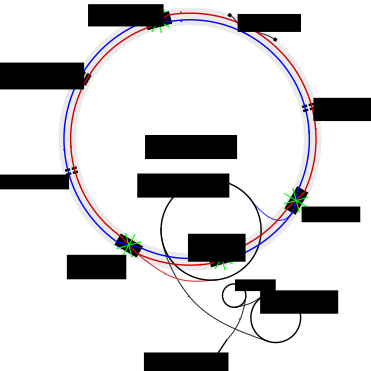
\includegraphics[width=0.9\textwidth]{lhc}
    \caption{Schematic illustration of the \acs{CERN} accelerator complex\cite{Ley:CERNAccelerators,Caron:LHCLayout,DeMelis:CERNacceleratorcomplex}. Protons first pass through several stages of preacceleration within the \ac{LINAC} 2, \ac{PS}, the \ac{PSB} and the \ac{SPS}. Eventually, they are injected into the \ac{LHC} where they circulate in opposite directions. The two beams are further accelerated in radio-frequency cavities and their shape is restored within the cleaning sections of the ring. At each revolution, some of the protons are brought to collision within one of the four experiments \acs{CMS}, \acs{ATLAS}, \acs{LHCb} and \acs{ALICE}. Once they are not needed anymore, the remaining protons can be dumped into massive metal blocks at the dump site.
    %Note that the accelerator sizes and positions are not to scale.
    }
    \label{fig:LHC}
\end{figure}

This work will focus on the \ac{CMS} experiment, which will be discussed in the next sections.

\section{The Compact Muon Solenoid}
The \ac{CMS} detector consists of multiple particle detector subsystems surrounding the interaction point.
Its goal is to measure outgoing particles created at proton-proton collisions.
The observed properties include particle type, direction, momentum, energy and charge. Each of the detector subsystems is dedicated to measuring one or more of these characteristics. The subsystems are read out electronically and the data are later analyzed on a computing grid.

An overview of the detector can be seen in \fref{fig:CMS_slice}. The discussion of the detector subsystems in the following sections is based on \cite{Chatrchyan:CMSexperimentCERN} if not explicitly stated otherwise.

\begin{figure}
    \centering
    \raisebox{0.31\height}{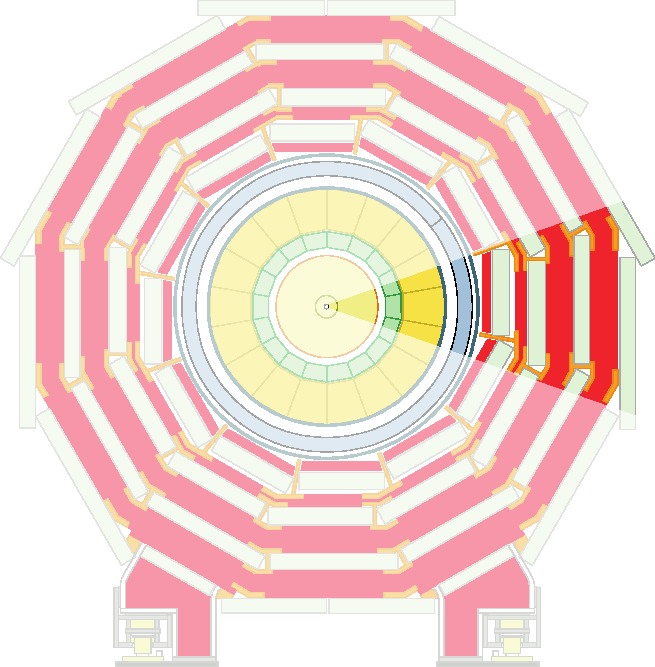
\includegraphics[width=0.3\textwidth]{cms_slice_context}}
    \hspace{0.02\textwidth}
    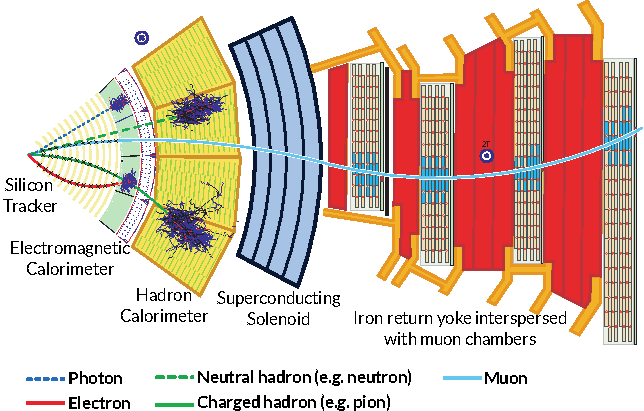
\includegraphics[width=0.65\textwidth]{cms_slice}
    \caption{Slice through the CMS detector barrel. From left to right the following subsystems are drawn: the silicon tracker, the electromagnetic and hadron calorimeter, the superconducting solenoid coil, and the iron return yoke with the muon chambers. The solid lines represent charged particles which are bend due to the magnetic field\cite[modified]{Davis:CMSSlice}.}
    \label{fig:CMS_slice}
\end{figure}

\subsection{Detector Geometry and Coordinates}
In a region starting at \SI{23}{\m} before the detector, both beam pipes are united\cite{Evans:LHCMachine}. The proton groups traveling in opposite directions share the same beam pipe, which defines the $z$-axis of the detector coordinate system. The collisions occur approximately at the interaction point at $z = 0$.
The detector forms a barrel around the beam pipe. The barrel is subdivided into seven slices: five evenly sized \emph{wheels} and one so-called \emph{endcap} on each open side of the barrel. The central wheel is centered at $z = 0$.
Detector layers in the wheels are mostly arranged in a cylindrical manner around the beam pipes, while the layers in the endcaps are mounted orthogonally to the beam pipe.

The direction of an outgoing particle originating in the interaction point can be characterized either using right-handed cartesian coordinates $(x, y, z)$ or a spherical coordinate system $(\phi, \theta)$. The $x$-axis connects the interaction point with the center of the \ac{LHC} ring. The $y$-axis is perpendicular to the other axes, pointing upwards. Regarding spherical coordinates, the azimuthal angle $\phi$ is measured in the $x$-$y$ plane with $\phi = 0$ along the $x$-axis. $\theta$ indicates the polar angle between the $z$-axis and the direction of interest.
However, $\theta$ is rarely used because it is not invariant under Lorentz-boosts in the $z$ direction. Instead, the Lorentz-invariant pseudo-rapidity $\eta \defeq -\ln\left[\tan\left(\frac{\theta}{2}\right)\right]$ is used to describe the angular separation between a particle and the beam pipe. The detector components in context of $\eta$ ranges can be found in \fref{fig:cms_quadrant}.

To indicate angular separation between particles, the quantity $R = \sqrt{\Delta \eta^2 + \Delta \phi^2}$, which is Lorentz-invariant, can be defined. $\eta$ and $R$ will be relevant in context of particle reconstruction.

\begin{figure}
    \centering
    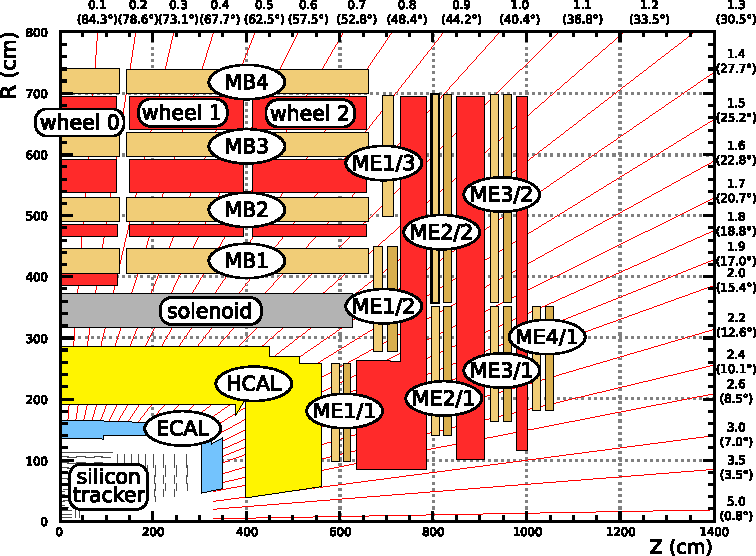
\includegraphics[width=0.8\textwidth]{cms_quadrant}
    \caption{Schematic view of a CMS quadrant, taken from \cite{CMSCollaboration:AligningCMSMuon}. Besides the angle $\theta$, the values for $\abs{\eta}$ are shown around the frame. This illustration focuses on the muon system, which consists of barrel (MB) and endcap (ME) stations. It extends to $\abs{\eta} = \num{2.4}$.}
    \label{fig:cms_quadrant}
\end{figure}

\subsection{Bunch Crossings and Pile-Up}
\label{sec:pileup}

For acceleration reasons, protons in the \ac{LHC} are grouped into packets called \emph{bunches}. At the interaction point, proton bunches from both directions collide every \SI{25}{\nano\second}, defining the so-called \emph{bunch crossing}. During each bunch crossing, multiple proton pairs may interact with each other. This multitude of collisions is called \emph{pile-up effect}.

Similarly, the collision of a single proton pair may result in multiple partons interacting with each other. This ambiguity is resolved by only analyzing the interaction with the highest momentum transfer, called \emph{hard interaction}. Other interactions contribute to the so-called \emph{underlying event}.

\subsection{Subsystems}
\subsubsection{Inner Tracking System}
The \emph{inner tracking system}\cite{Karimaeki:CMStrackersystem} is used for precise measurements of the direction and curvature of charged particles. 
It is composed of silicon semiconductor pixel layers surrounded by strip modules.

Each pixel cell consists of a silicon semiconductor in reverse bias direction. Charged particles passing through the semiconductor induce ionization and thus allow small currents to flow. These currents are amplified and read out by dedicated electronics. There are about \num{66} million pixel cells, each with a size of $\SI{100}{\micro\meter} \times \SI{150}{\micro\meter}$, allowing for a high spatial resolution.

The strip modules function similarly to the pixel cells. For reduced production costs, typical cell sizes are $\SI{10}{\centi\meter} \times \SI{80}{\micro\meter}$. There are \num{24244} silicon strips in the tracker.

A very high spatial resolution around the interaction point is necessary for finding the origin of decay products. This is achieved by tracing the particle tracks back to the location of their parent particles. The information is later used to discard particle tracks originating in pile-up  events or the underlying event (see \fref{sec:pileup}), as well as for identifying decays of \PB-mesons (see \fref{sec:b_tagging}).

\subsubsection{Electromagnetic Calorimeter}
\label{sec:ecal}
The goal of the \acfi{ECAL}\cite{CMS:CMSelectromagneticcalorimeter} is to measure the energy of outgoing electrons, positrons and photons. 

It consists of multiple layers of dense, transparent lead tungstate ($\textup{PbWO}_4$) crystals with a total thickness of \num{25} radiation lengths. Within these crystals, high energetic electrons and photons cause electromagnetic cascades: Electrons emit photons in the process of bremsstrahlung, while photons convert to electron-positron pairs in the process of pair-production.
This leads to large numbers of lower-energy electrons and photons, until the electron energy loss is dominated by ionization losses and the photon energy is below the pair-production threshold of $2 \si{\electronmass} = \SI{1022}{\keV}$.
Low energetic photons and those emitted by ionization or excitation are eventually registered using photodiodes. The initial particle energy is calculated from the light yield\cite{ParticleDataGroup:ReviewParticlePhysics}.

The energy resolution of the \ac{ECAL} has been studied on $\PZ \to \Pe + \Pe$ and $\PH \to \Pgamma \Pgamma$ simulations. The electron energy resolution (at $E_\text{T} \approx \SI{45}{\GeV}$)
is below \SI{2}{\percent} in the center of the barrel and \SIrange{2}{5}{\percent} elsewhere. The photon resolution (at $E_\text{t} \approx \SI{60}{\GeV}$) has been determined to be below \SI{3}{\percent} in the barrel and \SIrange{2}{5}{\percent} in the endcaps\cite{CMSCollaboration:Energycalibrationresolution}.

\subsubsection{Hadron Calorimeter}
In combination with the \ac{ECAL}, the energy of hadrons produced during the collision is measured by the  \acfi{HCAL}\cite{CMS:CMShadroncalorimeter}. 

It is designed as a sampling calorimeter with alternating layers of brass absorbers and plastic scintillator tiles. Hadrons passing through the calorimeter scatter on nuclei of the denser brass absorbers and cause hadronic showers \cite{ParticleDataGroup:ReviewParticlePhysics}.

The shower products are detected via scintillation. In the plastic scintillators, passage of charged particles excites electrons of the scintillator. During subsequent deexcitation, optical photons are emitted, which are guided through wavelength-shifting fibers to photodiodes. 

Because of the short nuclear interaction lengths in the absorber material, sampling calorimeters are more space efficient than homogeneous calorimeters.
However, as some of the energy is deposited within the absorber material, the total shower energy can only be estimated from the scintillation light. Overall, the \ac{HCAL} has a thickness of \numrange{7}{11} interaction lengths, depending on $\eta$.

Similarly to the electromagnetic calorimeter, a high resolution can be achieved only as long as the showers do not leak out of the calorimeter. 

\subsubsection{Solenoid Magnet}
The \ac{CMS} solenoid magnet\cite{CMS:CMSmagnetproject} is designed to deliver a magnetic field strength of \SI{4}{\tesla}. This is achieved by cooling the \SI{220}{\tonne} cold mass to \SI{4.6}{\kelvin}, such that the NbTi wires become superconducting and the current can reach up to \SI{19.5}{\kilo\ampere}.
The magnet surrounds the calorimeters and has a diameter of \SI{6}{\meter}. Within the coil, the magnetic field is approximately uniform with the field lines being parallel to the beam pipe. Outside, the magnetic flux is returned using an iron yoke, which is interspersed with the muon system.

Particles passing the field are subject to the Lorentz force which subsequently bends their tracks into helices. This effect allows to distinguish between charged and neutral particles and enables measurement of particle momenta.

\subsubsection{Muon System}
The goal of the muon system\cite{CMS:CMSmuonproject} is to detect muons and measure their tracks, from which the muon momenta are calculated.

Because of their high mass compared to electrons, muons are less affected by the electromagnetic fields within matter, reducing their radiative losses. This makes them the only detectable particles to pass through all inner detector subsystems as well as the solenoid coil.
For this reason, the muon system is the outermost part of the detector. It surrounds the solenoid coil and consists of \emph{resistive plate chambers} (\acsu{RPC}s), \emph{drift tubes} (\acsu{DT}s) in the barrel section and \emph{cathode strip chambers} (\acsu{CSC}s) in the endcaps. The muon barrel section extends in $\abs{\eta}$ up to \num{1.2}, the endcap region lies between $\abs{\eta}$ of \num{0.9} and \num{2.4}. In the range between \num{0.9} and \num{1.2}, the muon systems overlap.

Drift tubes have a length of about \SI{2}{\meter} and a cross section of $\SI{13}{\milli\meter} \times \SI{42}{\milli\meter}$. In the center of each tube, there is an anode wire. Between the wire and the tube walls exists a high electric potential. The tubes are filled with a gas mixture. 
As the charged muons pass through the gas, they ionize a few of the gas atoms. The released electrons accelerate along the electric field lines and induce secondary ionizations. Eventually, the accumulated charges are deposited in the anode wires and are measurable as current spike\cite{ParticleDataGroup:ReviewParticlePhysics}.
By measuring the drift time and combining results from several layers, a spatial resolution of less than \SI{100}{\micro\meter} can be achieved. However, determining the location in the wire direction is not possible with this arrangement.

In the endcap region, the muon system consists of cathode strip chambers instead of drift tubes. \acp{CSC} are gaseous detectors that contain several wires and cathode strips that are aligned orthogonally and read out separately. \acp{CSC} do not make use of drift effects, therefore are able operate under non-uniform magnetic fields and at high rates of muons, which makes them suited for use in the endcap region.

In both barrel and endcap, the \acp{DT} and \acp{CSC} are complemented with \acp{RPC}. Similarly to \acp{DT} and \acp{CSC}, \acp{RPC} are gaseous detectors, but are operated in avalanche mode. They possess a low spatial resolution but an excellent timing resolution, which helps to assign tracks to a bunch crossing.

The overall muon momentum resolution has been determined from measurements of cosmic muons and is approximately \SI{7}{\percent} for a \pT range of \SIrange{350}{2000}{\GeV}\cite{CMSCollaboration:PerformanceCMSmuon}.

\subsection{Triggering}
\label{sec:triggering}
As mentioned in \fref{sec:pileup}, the \ac{LHC} delivers collisions about every \SI{25}{\nano\second}, resulting in around \num{40} million events per second. Even with a raw event size of about \SI{500}{\kilo\byte}\cite{CMSCollaboration:CMStriggersystem}, storing all events would require a bandwidth of \SI{20}{\tera\byte\per\second}. Neither the read-out chips of the submodules nor the computer network between the detector and storage can currently handle data traffic of this magnitude.

Therefore, the rate of events accepted for storage and analysis has to be drastically reduced. This is the task of the \emph{triggering system}. Based on the physics content, statistics and bandwidth restrictions, triggers decide whether or not to store an event to disk.

Triggering is implemented in a two step process: First, the \acfi{L1} trigger is consulted. It is implemented in dedicated hardware and uses information from the calorimeters and the muon system to reject low-energetic events. Events passing \ac{L1} will be read out, temporarily stored and further evaluated by the \acfi{HLT}. The \ac{HLT} is implemented in software and runs on computers next to the detector cavern. It has access to the full detector information to decide whether an event is eventually to be stored or rejected\cite{CMSCollaboration:CMStriggersystem}.

\subsection{The Computing Grid}
Reconstruction and analyses are ran on the stored events. For this purpose, the \acfi{WLCG} project was founded, which consists of several computing facilities operated by the \ac{CERN} member states.

The facilities are organized in layers called \emph{tiers}. There are two tier 0 computing centers, one at the \ac{CERN} data center in Geneva and one at the Wigner Research Centre for Physics in Budapest, which store and reconstruct raw data. From there, the data are distributed to one of the 13 tier 1 data centers worldwide, where they are further processed, stored for safe-keeping and distributed to tier 2 facilities.

There are about 160 tier 2 computing centers, most of which are operated by universities and other scientific institutes. Their task is to provide computing power for event generation and analyses\cite{CERN:Gridsystemtiers,WLCG:Tiercentres}. One of these tier 2 centers is operated at the physics department of the RWTH Aachen University, currently providing around \num{5200} processing cores and \SI{3}{\peta\byte} of storage\cite{UniRWTHAachenIII.PhysikalischesInstitut:GridComputing}. 
